\subsection{Rivelatore di neutroni}
Essendo particelle neutre, i neutroni non possono essere rivelati con \emph{detectors} che sfruttano il principio della ionizzazione, perciò una strumentazione dedicata è necessaria.
I rivelatori di neutroni sono basati sulla rivelazione di prodotti secondari (fotoni, particelle cariche) dalle reazioni nucleari indotte dall'urto del neutrone su elementi tipo $^{10}$B o $^6$Li. Questo sistema di rivelazione è efficace solo per i neutroni termici, e proprio per questo è ideale per la nostra misura sul flusso di neutroni. 
Proponiamo due sistemi di rivelazione: essi hanno pregi e difetti che richiedono un approfondimento maggiore per scegliere quale utilizzare nell'esperienza (\emph{che svolgeremo qualora il progetto venisse approvato}). 

Un sistema utilizza come rivelatore il dosimetro CT007-T della GammaGuard. Il dosimetro comunica tramite Bluetooth con una applicazione per Android, dove i dati (compresi data e coordinate GPS) vengono conservati. Il salvataggio dei dati viene eseguito attraverso comandi manuali alla fine dell'acquisizione, perciò c'è la necessità di un cellulare che rimanga funzionante in volo e dopo l'atterraggio. Non poter salvare automaticamente i dati è il difetto principale di questo sistema.

La seconda proposta prevede di utilizzare un rivelatore della ditta Scionix che accoppia un rivelatore di fotoni a semiconduttore a un cristallo di iodurio di $^6 $Li drogato con europio. Il sistema viene letto da un circuito elettronico simile a quello già montato per il rivelatore di particelle cariche (e sfrutta parte di quella elettronica). Essendo realizzato su misura, questo rivelatore è potenzialmente più affidabile per i nostri scopi; tuttavia questo sistema risulta più complesso del primo, che è già pronto all'uso. 

\begin{figure}
    \centering
    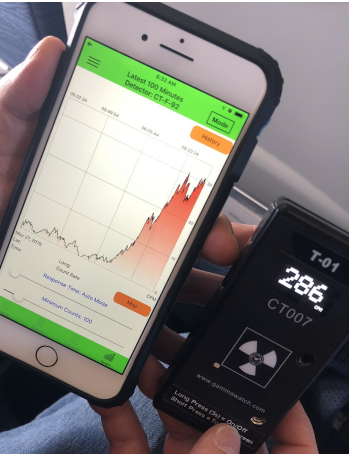
\includegraphics[width=0.2\textwidth]{CT007-T.png}
    \quad
    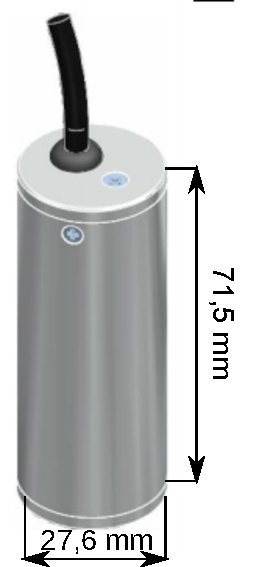
\includegraphics[width=0.12\textwidth]{Scionix.pdf}
    \caption{A sinistra: foto del sistema CT007-T + cellulare; a destra: disegno del rivelatore Scionix.}
    \label{fig:my_label}
\end{figure}
